\documentclass[english]{article}
\usepackage[T1]{fontenc}
\usepackage[latin9]{inputenc}
\usepackage{float}
\usepackage{graphicx}
\usepackage{esint}
\usepackage{geometry}             
\geometry{letterpaper}   
\usepackage{listings}
\usepackage{color} %red, green, blue, yellow, cyan, magenta, black, white
\definecolor{mygreen}{RGB}{28,172,0} % color values Red, Green, Blue
\definecolor{mylilas}{RGB}{170,55,241}
\makeatletter
\@ifundefined{showcaptionsetup}{}{%
 \PassOptionsToPackage{caption=false}{subfig}}
\usepackage{subfig}
\makeatother
\usepackage{babel}
\begin{document}
\title{MLPR Assignment}
\author{Paridhi Mishra (s1549106)}
\date{24th Nov 2015}
\maketitle
\section*{1. The Next Pixel Prediction Task}
\subsection*{Q1 Data preprocessing and visualization }
\subsection*{(a)}
\begin{figure}[h!]
  \caption{Histogram}
  \centering
    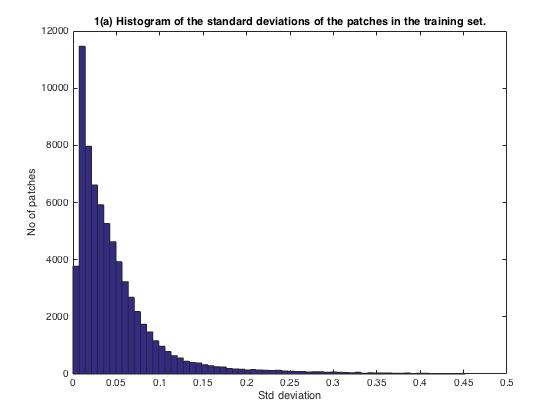
\includegraphics[width=0.8\textwidth]{fig_1_1_a.jpg}
\end{figure}

Observations from histogram:

1. Many patches have low deviations eg. roughly 3900 patches have ~0 std deviations whereas
 roughly 11,000 out of 70,000 patches have ~0.01 std deviation, indicating
 that a lot of these pixels values are similar, (smooth patches).
 
2. Since we assume all patches with std dev < 0.063(4/63) are flat
 patches, from the plot is can be inferred that more than half of the patches
 are flat.
 
3. Some patches have very high deviations as well. of the standard deviations of the patches in the training set indicating that they can help in modelling (interesting patches).

Here 64 bins is used because the image has been discretized by 64 grey
scales and this way each bin will plot each grey scale value for the image.

\subsection*{(b)}
A simple way is to predict a flat patch is by comparing the y(j) pixel with the mean of 
all pixels in this same patch. It can also be done by comparing the mean of all pixels of this 
patch with the mean of x(j,end), x(j,end-34) and y(j). If both values are very similar, the chances of 
the patch being flat is high.

\subsection*{(c)}
(c) Figures for flat and non-flat image patch is given below.
Matlab code at the end of this section.

\begin{figure}[h!]
  \caption{}
  \centering
    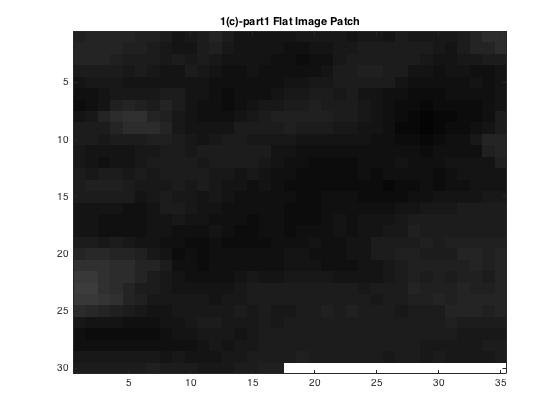
\includegraphics[width=0.8\textwidth]{fig_1_1_c_1_flat.jpg}
\end{figure}
\begin{figure}[h!]
  \caption{}
  \centering
    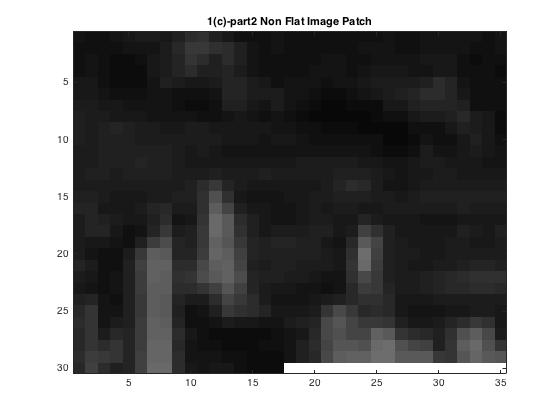
\includegraphics[width=0.8\textwidth]{fig_1_1_c_2_nonflat.jpg}
\end{figure}

\medskip
\subsection*{Matlab Code - Q1.1}
\lstset{language=Matlab,%
    %basicstyle=\color{red},
    breaklines=true,%
    morekeywords={matlab2tikz},
    keywordstyle=\color{blue},%
    morekeywords=[2]{1}, keywordstyle=[2]{\color{black}},
    identifierstyle=\color{black},%
    stringstyle=\color{mylilas},
    commentstyle=\color{mygreen},%
    showstringspaces=false,%without this there will be a symbol in the places where there is a space
    numbers=left,%
    numberstyle={\tiny \color{black}},% size of the numbers
    numbersep=9pt, % this defines how far the numbers are from the text
    emph=[1]{for,end,break},emphstyle=[1]\color{red}, %some words to emphasise
    %emph=[2]{word1,word2}, emphstyle=[2]{style},    
}
\lstinputlisting{mlpr1_1.m}

\medskip

\subsection*{Q1.2 Linear regression with adjacent pixels}

\begin{figure}[h!]
  \caption{.}
  \centering
    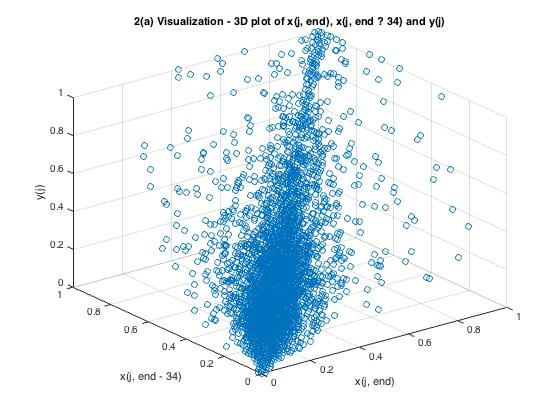
\includegraphics[width=0.8\textwidth]{fig_1_2_a.jpg}
\end{figure}

\medskip

\subsection*{(a)}
The 3D plot of x(j, end), x(j, end ? 34) and y(j) is presented in Figure 4. For this 3D plot, the data has been subsampled by taking every other row from both datasets Both subsampled sets had roughly 8600 instances after this operation.Strong positive linear correlations between all the 3 pixels are visible in this scatter plot. Both pixels x(j;end) and x(j:end-34) can help in predicting pixel y(j) because of this  behaviour. This also indicates that linear regression might be a good technique to explore  the interesting statistical trends in this image.
\subsection*{(b)}
Bias weight has been added as 3nd column to matrix of  x(j, end) and x(j, end - 34),
and denoted as X. Let Y represent the vector for y(j) values.
MLE solution
$\textbf{w}$ = $\textbf{(inv}$$\textbf{(X}^\top$ $\textbf{X))}$$\textbf{X}^\top$$\textbf{y}$

The inv() function above is exponent to the power -1 (the inverse function). 
\subsection*{(c)}
The linear regression predictor is implemented in matlab as shown in code below.
The weight vector values are: w = [ 0.46064 ; 0.52412 ; 0.00256 ].The root mean squared error on the training and test sets are RMSE training = 0.0506  and  RMSE test = 0.0503 . Both values are very similar which indicates that the model is a good model and the training data was not over fitted. Had that been the case, RMSE of the test would have been much higher that RMSE of the training set.

The regression surface of this linear predictor in 3-D using Matlab function surf() is in Figure 5 below. From this plot, the data is linearly separable as almost all test points like above this regression surface. which means that the linear classifier is successful in predicting the pixel values(y(j)) given the training set of pixels.

\begin{figure}[h!]
  \caption{}
  \centering
    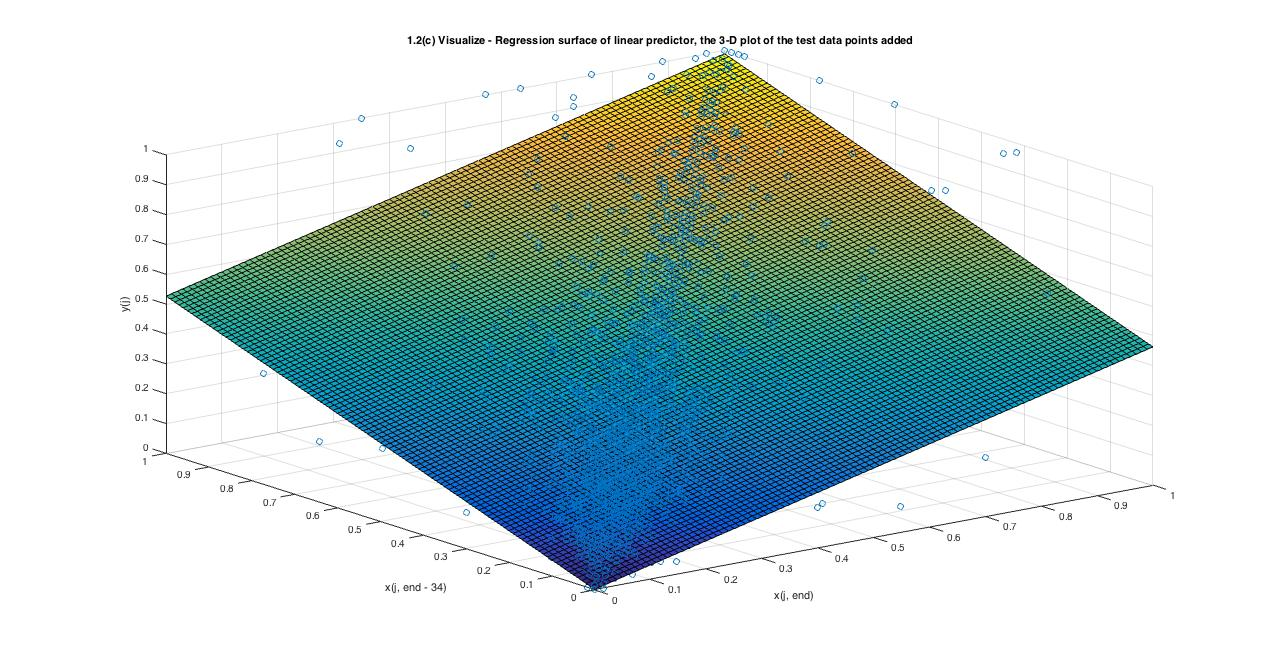
\includegraphics[width=0.8\textwidth]{fig_1_2_c.jpg}
\end{figure}
\medskip

\medskip

\lstset{language=Matlab,%
    %basicstyle=\color{red},
    breaklines=true,%
    morekeywords={matlab2tikz},
    keywordstyle=\color{blue},%
    morekeywords=[2]{1}, keywordstyle=[2]{\color{black}},
    identifierstyle=\color{black},%
    stringstyle=\color{mylilas},
    commentstyle=\color{mygreen},%
    showstringspaces=false,%without this there will be a symbol in the places where there is a space
    numbers=left,%
    numberstyle={\tiny \color{black}},% size of the numbers
    numbersep=9pt, % this defines how far the numbers are from the text
    emph=[1]{for,end,break},emphstyle=[1]\color{red}, %some words to emphasise
    %emph=[2]{word1,word2}, emphstyle=[2]{style},    
}
\subsection*{Matlab Code - Q1.2- Linear Regression - 2 variables}
\lstinputlisting{mlpr1_2.m}

\medskip
\subsection*{Q1.3 RBF regression with adjacent pixels}
\subsection*{(a)}
The RBF model was tried with following number of basis functions {5, 10, 15, 20, 25, 30}.
using crossval function. The plot for  the cross-validation RMSE against the number of RBFs used, 
is shown in Figure 6 below. Hence best model selected is for nbf = 10. The matlab code which
implements this RBF model is shown below.
\begin{figure}[h!]
  \caption{}
  \centering
    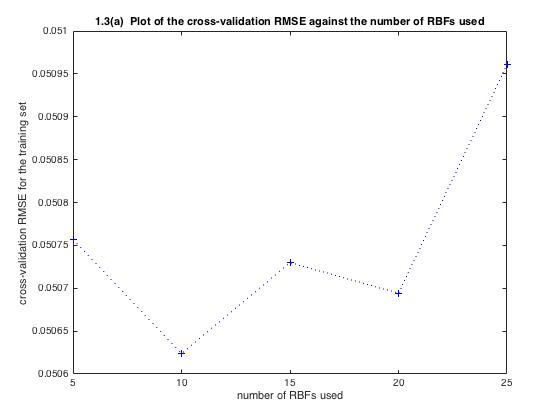
\includegraphics[width=0.8\textwidth]{fig_1_1_3.jpg}
\end{figure}

\subsection*{(b)} 
Choosing nbf = 10 (for which rmse is ~ 0.05063), the RBF network is trained using all the non-flat training data . The values are -RMSE training = 0.0498  and RMSE test = 0.0526. Again, both the values are very close indicated  a good fit for this model over given data. There is a slight improvement in RMSE compared to the  previous linear regression model.

\lstset{language=Matlab,%
    %basicstyle=\color{red},
    breaklines=true,%
    morekeywords={matlab2tikz},
    keywordstyle=\color{blue},%
    morekeywords=[2]{1}, keywordstyle=[2]{\color{black}},
    identifierstyle=\color{black},%
    stringstyle=\color{mylilas},
    commentstyle=\color{mygreen},%
    showstringspaces=false,%without this there will be a symbol in the places where there is a space
    numbers=left,%
    numberstyle={\tiny \color{black}},% size of the numbers
    numbersep=9pt, % this defines how far the numbers are from the text
    emph=[1]{for,end,break},emphstyle=[1]\color{red}, %some words to emphasise
    %emph=[2]{word1,word2}, emphstyle=[2]{style},    
}
\subsection*{Matlab Code - Q1.3 - RBF}
\lstinputlisting{mlpr1_3.m}


\subsection*{Q1.4 Linear regression with all pixels }
Extending the model and implementing the linear regression with all pixels,
RMSE training = 0.0456  and RMSE test = 0.0371 .Compared to its simpler version of linear model, it performs better on both the training and test sets, but marginally only. Given that so many extra
parameters were provided for this model, the performance has not improved significantly. It indicates
that the 2 previous pixels alone can predict the target pixel in a satisfactory manner.
Compared to the RBF model too, if performs a little better as seen from the RMSE values, but since
there is no  concrete proof that it is a better model that RBF.

\lstset{language=Matlab,%
    %basicstyle=\color{red},
    breaklines=true,%
    morekeywords={matlab2tikz},
    keywordstyle=\color{blue},%
    morekeywords=[2]{1}, keywordstyle=[2]{\color{black}},
    identifierstyle=\color{black},%
    stringstyle=\color{mylilas},
    commentstyle=\color{mygreen},%
    showstringspaces=false,%without this there will be a symbol in the places where there is a space
    numbers=left,%
    numberstyle={\tiny \color{black}},% size of the numbers
    numbersep=9pt, % this defines how far the numbers are from the text
    emph=[1]{for,end,break},emphstyle=[1]\color{red}, %some words to emphasise
    %emph=[2]{word1,word2}, emphstyle=[2]{style},    
}
\subsection*{Matlab Code - Q1.4 - Linear Regression - all pixels}
\lstinputlisting{mlpr1_4.m}

\section*{Q1.5 Neural Network with all pixels }
\subsection*{(a)} 

Using the well trained MLP provided, a neural network was built with 10 hidden units. The  
RMSE training = 0.0333  and RMSE test = 0.0473.

Comparing its RMSEs with those from linear regression, there is a small difference only. What is noticeable is that the linear regression model seems to be less overfitting that the NN since the difference if test and training values is smaller. At the same time, the RMSE of training of NN is better than linear model which indicates makes it harder to compare both these models. 

\subsection*{(b)}

Using first 5000 data points to train the MLP and running the training 5 times using different random seeds, the resulting RMSE's are given below. The Matlab code is provided at the end of the section.

All the training and test RMSE values for the small dataset (first 5000 points) are higher that what was 
observed in 1.5.a. Even though different initial values (random seeds) were used for 5 different times, it did not show improvement  This suggests that this subset of data taken might not be very representative of the original dataset. It is also possible that since NNs adapts its network as it learns from data, the lesser data it saw in this part is the reason for higher error values. If so, then it is expected to perform better with larger datasets and over time.
\\
\\
Training RMSE		Test RMSE
\\
0.0475 \hspace{2cm}0.0499
\\
0.0488 \hspace{2cm}0.0515
\\
0.0485 \hspace{2cm}0.0515
\\
0.0486 \hspace{2cm}0.0527
\\
0.0489 \hspace{2cm}0.0526

\lstset{language=Matlab,%
    %basicstyle=\color{red},
    breaklines=true,%
    morekeywords={matlab2tikz},
    keywordstyle=\color{blue},%
    morekeywords=[2]{1}, keywordstyle=[2]{\color{black}},
    identifierstyle=\color{black},%
    stringstyle=\color{mylilas},
    commentstyle=\color{mygreen},%
    showstringspaces=false,%without this there will be a symbol in the places where there is a space
    numbers=left,%
    numberstyle={\tiny \color{black}},% size of the numbers
    numbersep=9pt, % this defines how far the numbers are from the text
    emph=[1]{for,end,break},emphstyle=[1]\color{red}, %some words to emphasise
    %emph=[2]{word1,word2}, emphstyle=[2]{style},    
}
\subsection*{Matlab Code - Q1.5}
\lstinputlisting{mlpr1_5.m}


\subsection*{Q1.6 Discussion}


Above we have considered linear regression and RBF network using 2 neighbouring
pixels, and linear regression and a neural network on all pixels. 

When comparing with only 2 pixels (2 variables as input data), the linear regression is expected to perform very well as 
Compare these methods
Especially for all pixels case, NN has the advantage that it can model non linearities in 
multiple pixels automatically when compared to a linear regression model which implements
a statistical model . For example incase the training data has noise, NN is better in mapping
 hidden and nonlinear input-output dependencies ..But with the freedom of adding multiple hidden layers and nodes, the NN is also more prone to overfitting of the data that linear model. 

In this particular task of pixel prediction for image compression, NN model minimizes the training 
root mean squared error, thus the neural networks prediction, leads to better results.

Briefly, what experiment would you try next if you wanted to improve on these
predictors?

As number of pixels grow, I would like to try which of above two models handle
large numerical data better.
Also, once implemented, which model is better at adjusting with the changes, say 
for example accomodating the historical data 
The next experiment I would try is changing the dataset and running the models on these
new datasets since comparing the models on a single dataset can be dangerous.

Due to the complexities which increase as the network and hidden layers increase in
an adaptive NN model, I would like to compare the models in terms of execution time.It might
be possible that the NN model is unnecessarily slow for this task.

\section*{Q.2. Robust modelling}


\subsection*{Q2.1 Fitting the baseline model}


\subsection*{(a)}

The bias feature was added in the logistic regression model by augmenting the data and adding
an extra dimension. The bias weight bw (d+1) recorded is 


\subsection*{(b)}
(b) Maximizing the likelihood

Test set
Accuracy = 0.3194
Mean Log Probability = -0.7140
Std error = 0.0116
\\
Training set
Accuracy = 0.2977
Mean Log Probability = -0.7311
Std error  = 0.0057


Performance of predictions on training and test

We know that a baseline that predicts P(y|x)=0.5 makes no assumptions
about the data, so it will have error of 0.5 for every prediction.  Mean
probability, however, will predict closer to the label that it predicts
as more common.  So long as the label it predicts as more common IS more
common, a baseline that uses mean probability will be better.


\subsection*{(c)}
(c) Limited training data

Avg log probability = -0.6196
Because a small training set was used, many of the weights in the weight
vector quicky minimize to either 0 or 1, indicating that in this small 
training set, all feature vectors with a certain value for a certain
feature had the same label.  In our concrete text classification example,
this would indicate that for instance that only sports-labelled documents 
contained the word "pass."
When this weight vector is used to classify a document, the linear
regressor returns values of zero or one.  This is an artifact of weight
vectors that over-generalize the likelihood of seeing a given feature in a
document of a given label, but the effect is to make the regressor entirely
certain of a document's label.  If the regressor returns a probability of 0
for any of the documents in the test set, then the mean log probability
becomes -Inf +/- NaN.


\lstset{language=Matlab,%
    %basicstyle=\color{red},
    breaklines=true,%
    morekeywords={matlab2tikz},
    keywordstyle=\color{blue},%
    morekeywords=[2]{1}, keywordstyle=[2]{\color{black}},
    identifierstyle=\color{black},%
    stringstyle=\color{mylilas},
    commentstyle=\color{mygreen},%
    showstringspaces=false,%without this there will be a symbol in the places where there is a space
    numbers=left,%
    numberstyle={\tiny \color{black}},% size of the numbers
    numbersep=9pt, % this defines how far the numbers are from the text
    emph=[1]{for,end,break},emphstyle=[1]\color{red}, %some words to emphasise
    %emph=[2]{word1,word2}, emphstyle=[2]{style},    
}
\subsection*{Matlab Code - Q2.1 - Fitting the baseline model}
\lstinputlisting{m1.m}

\subsection*{Q2.2 Label noise model}


\subsection*{(a)}
(a) Modifying the likelihood:

Functions created which return log likelihood of this model, given data are:
log_like_noise_w()  and log_like_noise_e() w.r.t w and e. The called functions are
presented in the appendix for matlab code and the main calling code is presented at the
end of this section. Checkgrad.m routine has been used to check the gradients.
\subsection*{(b)}
(b) Fitting a constrained parameter: 

Create a function that evaluates the negative log-likelihood of the new model and
evaluates the derivatives with respect to w and a. Hence fit both w and a. You are
advised to wrap the function from the previous part, rather than starting from scratch.
Report the fitted noise level e=?(a).
Given that the test labels were checked more carefully, predict them using the newly
fitted weights but using the original model (1). Report and interpret the new test
accuracy and mean log probability.

\lstset{language=Matlab,%
    %basicstyle=\color{red},
    breaklines=true,%
    morekeywords={matlab2tikz},
    keywordstyle=\color{blue},%
    morekeywords=[2]{1}, keywordstyle=[2]{\color{black}},
    identifierstyle=\color{black},%
    stringstyle=\color{mylilas},
    commentstyle=\color{mygreen},%
    showstringspaces=false,%without this there will be a symbol in the places where there is a space
    numbers=left,%
    numberstyle={\tiny \color{black}},% size of the numbers
    numbersep=9pt, % this defines how far the numbers are from the text
    emph=[1]{for,end,break},emphstyle=[1]\color{red}, %some words to emphasise
    %emph=[2]{word1,word2}, emphstyle=[2]{style},    
}
\subsection*{Matlab Code - Q2.2}
\lstinputlisting{mlpr2_2.m}


\subsection*{ Q2.3 Hierarchical model and MCMC}


\subsection*{(a)}

If a model were somehow able to predict every training label correctly, the binary 
noise variable from Eq 3 will become 0 and the log likelihood will behave as a 
model with no noise.
For w = 0, the likehihood will become sum(log(1/(1+e^0))) = sum(log(0.5)) = N*(-0.6)
\\
 N is the number of training/test samples.

\subsection*{(b)}

Putting w, e and log lambda into a single vector, and writing a wrapper to the log posterior
function to evaluate  Eq(6), slice sample fn was called. Step out values was toggled
between false and true, and a number of combinations of width, burn and N were tried.
For initialization of the row vector with {e,lambda,w}, rand fn was called to set the values.

The function returned N samples of {e,lambda,w}. Plot of lambda against e is shown below.
Since the step-out was set to false, the function did not performed as expected.
  
\begin{figure}[h!]
  \caption{}
  \centering
    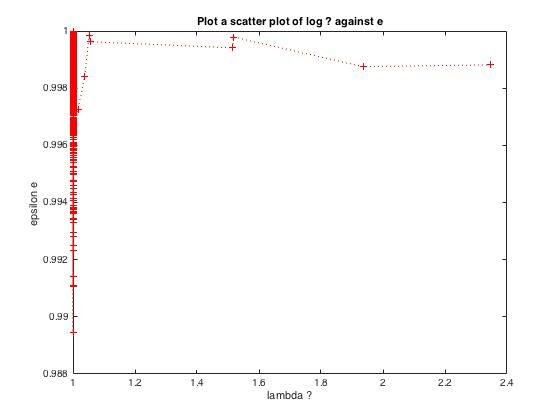
\includegraphics[width=0.8\textwidth]{last_fig.jpg}
\end{figure}
\subsection*{(c)}
The slice sampler was hung indefinitely with step out = true. All the samples returned with step-out = false are valid, even though the distribution is not as expected. These observations can be utilized as part of test sets of the same model. The values observed are  epsilon values are high - between 0.9 and 1.0 and the lambda values are between 1 and 3. Since the function did not complete the execution as expected, the comparison is not possible.

\lstset{language=Matlab,%
    %basicstyle=\color{red},
    breaklines=true,%
    morekeywords={matlab2tikz},
    keywordstyle=\color{blue},%
    morekeywords=[2]{1}, keywordstyle=[2]{\color{black}},
    identifierstyle=\color{black},%
    stringstyle=\color{mylilas},
    commentstyle=\color{mygreen},%
    showstringspaces=false,%without this there will be a symbol in the places where there is a space
    numbers=left,%
    numberstyle={\tiny \color{black}},% size of the numbers
    numbersep=9pt, % this defines how far the numbers are from the text
    emph=[1]{for,end,break},emphstyle=[1]\color{red}, %some words to emphasise
    %emph=[2]{word1,word2}, emphstyle=[2]{style},    
}
\subsection*{Matlab Code - Q2.3 - Hierarchial Model and MCMC}
\lstinputlisting{mlpr2_3.m}

\section*{Appendix A - Additional Code}

\lstset{language=Matlab,%
    %basicstyle=\color{red},
    breaklines=true,%
    morekeywords={matlab2tikz},
    keywordstyle=\color{blue},%
    morekeywords=[2]{1}, keywordstyle=[2]{\color{black}},
    identifierstyle=\color{black},%
    stringstyle=\color{mylilas},
    commentstyle=\color{mygreen},%
    showstringspaces=false,%without this there will be a symbol in the places where there is a space
    numbers=left,%
    numberstyle={\tiny \color{black}},% size of the numbers
    numbersep=9pt, % this defines how far the numbers are from the text
    emph=[1]{for,end,break},emphstyle=[1]\color{red}, %some words to emphasise
    %emph=[2]{word1,word2}, emphstyle=[2]{style},    
}

\lstinputlisting{log_posterior.m}
\medskip
\lstinputlisting{split_params.m}
\medskip
\lstinputlisting{init_params.m}
\medskip
\lstinputlisting{log_like_negative.m}
\medskip
\lstinputlisting{log_like_noise_w.m}
\medskip
\lstinputlisting{log_like_noise_e.m}
\medskip
\lstinputlisting{log_like_noise_a.m}




\section*{Appendix B - References}
\\
1.http://uk.mathworks.com/help/
\\
2.http://mlg.eng.cam.ac.uk/zoubin/tut06/mcmc.pdf
\\
3..http://homepages.inf.ed.ac.uk/imurray2/teaching


\end{document}
